\setcounter{definition}{0} \setcounter{property}{0} \setcounter{claim}{0} \setcounter{fact}{0} \setcounter{corollary}{0} \setcounter{figure}{0}
\section{Shortest Path Problem Revisited}

%%%We will design two algorithms, namely a dynamic programming algorithm and the Bellman-Ford algorithm,
%%%for shortest path problem in the presence of negative edge length.
%%%
%%%\subsection*{Negative Cycle}
%%%
%%%A negative cycle $C$ in a graph is a cycle with negative length, i.e., $l(C) := \sum_{e\in C} l(e) < 0$.
%%%In the presence of negative cycle, if we don't limit the number of edges
%%%in a path, then the length of a path could goes to negative infinity.
%%%In other words, the shortest path may not exist.
%%%Therefore, in a graph with negative edge length, we want to
%%%detect if there exists negative cycle.
%%%We will show that later on, both the dynamic programming algorithm
%%%and Bellman-Ford algorithm can be extended to detect negative cycle.
%%%
%%%A path $p$ in a graph is \emph{simple} if $p$ does not have repeating vertices.
%%%If a graph $G$ does not contain negative cycle, then 
%%%for any pair of vertices $u$ and $v$, if $u$ can reach $v$,
%%%then there always exists a {simple} shortest path from $u$ to $v$,
%%%as otherwise we can skip the cycle in it to get a better or same-length path.
%%%If all cycles in graph $G$ are positive then every shortest path is simple.
%%%
%%%\subsection*{Framework of Dynamic Programming Algorithm}
%%%
%%%A typical dynamic programming algorithm consists of following steps:
%%%\vspace*{-\topsep}
%%%\begin{enumerate}
%%%\item Define subproblems~(or equivalently, partition the search space into sub-spaces),
%%%$P_1, P_2, \cdots, P_n$; solving all these subproblems will solve the original problem.
%%%\item Develop a recursion for these subproblems. Formally, let $opt(P_k)$ be the optimal
%%%solution of $P_k$. A recursion is a function that calculates
%%%$opt(P_{k+1})$ using $opt(P_1), opt(P_2), \cdots, opt(P_k)$.
%%%\item Fill a \emph{dynamic programming table},
%%%in which each entry stores the optimal solution of a subproblem, 
%%%using above recursion.
%%%\end{enumerate}
%%%
%%%
%%%\subsection*{DP Algorithm for Shortest Path Problem}

Let's revisit the shortest path problem with possibly negative edge length.
Formally, given graph $G = (V, E)$ with edge length $l(e)$ for any $e\in E$~(note
that it could be that $l(e) < 0$) and source vertex $v\in V$,
to calculate the shortest path from $s$ to every $v\in V$.
Here we assume that $G$ does not contain negative cycle~(so
the shortest path exists for every vertex that is reachable from $s$).

We first define subproblems: define $dist(k,v)$ as the length
of the shortest path from $s$ to $v$ using at most $k$ edges;
the ``subproblem'' is then to calculate $dist(k,v)$.
These subproblems correspond to partition the ``search space''
in this way: define $X(v)$ as the set of all paths from $s$ to $v$ in $G$.
Define $X(k, v)$ as the set of all paths from $s$ to $v$ using
at most $k$ edges. Therefore, $dist(k,v)$ is the length
of the optimal path in $X(k,v)$.

Here's connection of these subproblems with the original problem.
\begin{fact}
If $G$ does not contain negative cycle, then $dist(|V| - 1, v) = distance(s, v)$ for every $v\in V$.
\end{fact}

\begin{figure}[h]
\centering{

\tikzset{every picture/.style={line width=0.75pt}} %set default line width to 0.75pt        

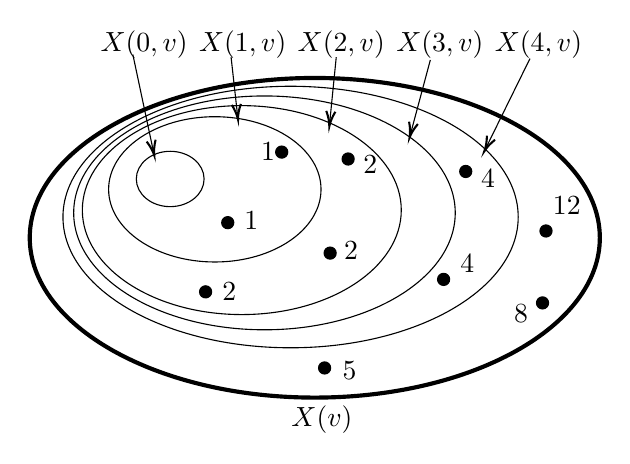
\begin{tikzpicture}[x=0.5pt,y=0.5pt,yscale=-1,xscale=1]
%uncomment if require: \path (0,327); %set diagram left start at 0, and has height of 327

%Shape: Ellipse [id:dp0428766556986383] 
\draw  [line width=1.5]  (59,177.5) .. controls (59,113.71) and (151.23,62) .. (265,62) .. controls (378.77,62) and (471,113.71) .. (471,177.5) .. controls (471,241.29) and (378.77,293) .. (265,293) .. controls (151.23,293) and (59,241.29) .. (59,177.5) -- cycle ;
%Shape: Ellipse [id:dp14451946279796424] 
\draw   (136,135) .. controls (136,123.95) and (146.97,115) .. (160.5,115) .. controls (174.03,115) and (185,123.95) .. (185,135) .. controls (185,146.05) and (174.03,155) .. (160.5,155) .. controls (146.97,155) and (136,146.05) .. (136,135) -- cycle ;
%Shape: Ellipse [id:dp2511588613225232] 
\draw   (116,142.5) .. controls (116,113.51) and (150.36,90) .. (192.75,90) .. controls (235.14,90) and (269.5,113.51) .. (269.5,142.5) .. controls (269.5,171.49) and (235.14,195) .. (192.75,195) .. controls (150.36,195) and (116,171.49) .. (116,142.5) -- cycle ;
%Shape: Ellipse [id:dp5415787744293407] 
\draw   (97,157.5) .. controls (97,115.8) and (148.6,82) .. (212.25,82) .. controls (275.9,82) and (327.5,115.8) .. (327.5,157.5) .. controls (327.5,199.2) and (275.9,233) .. (212.25,233) .. controls (148.6,233) and (97,199.2) .. (97,157.5) -- cycle ;
%Shape: Ellipse [id:dp42014218433161865] 
\draw   (83,162.5) .. controls (83,110.31) and (156.65,68) .. (247.5,68) .. controls (338.35,68) and (412,110.31) .. (412,162.5) .. controls (412,214.69) and (338.35,257) .. (247.5,257) .. controls (156.65,257) and (83,214.69) .. (83,162.5) -- cycle ;
%Flowchart: Connector [id:dp24980663040863116] 
\draw  [fill={rgb, 255:red, 0; green, 0; blue, 0 }  ,fill opacity=1 ] (198,165) .. controls (198.87,162.74) and (201.4,161.62) .. (203.66,162.49) .. controls (205.91,163.36) and (207.04,165.89) .. (206.17,168.15) .. controls (205.3,170.4) and (202.77,171.53) .. (200.51,170.66) .. controls (198.26,169.79) and (197.13,167.26) .. (198,165) -- cycle ;
%Flowchart: Connector [id:dp6930751898796546] 
\draw  [fill={rgb, 255:red, 0; green, 0; blue, 0 }  ,fill opacity=1 ] (237,114) .. controls (237.87,111.74) and (240.4,110.62) .. (242.66,111.49) .. controls (244.91,112.36) and (246.04,114.89) .. (245.17,117.15) .. controls (244.3,119.4) and (241.77,120.53) .. (239.51,119.66) .. controls (237.26,118.79) and (236.13,116.26) .. (237,114) -- cycle ;
%Flowchart: Connector [id:dp6974875632568183] 
\draw  [fill={rgb, 255:red, 0; green, 0; blue, 0 }  ,fill opacity=1 ] (425.5,223) .. controls (426.37,220.74) and (428.9,219.62) .. (431.16,220.49) .. controls (433.41,221.36) and (434.54,223.89) .. (433.67,226.15) .. controls (432.8,228.4) and (430.27,229.53) .. (428.01,228.66) .. controls (425.76,227.79) and (424.63,225.26) .. (425.5,223) -- cycle ;
%Flowchart: Connector [id:dp15058432994873683] 
\draw  [fill={rgb, 255:red, 0; green, 0; blue, 0 }  ,fill opacity=1 ] (182,215) .. controls (182.87,212.74) and (185.4,211.62) .. (187.66,212.49) .. controls (189.91,213.36) and (191.04,215.89) .. (190.17,218.15) .. controls (189.3,220.4) and (186.77,221.53) .. (184.51,220.66) .. controls (182.26,219.79) and (181.13,217.26) .. (182,215) -- cycle ;
%Flowchart: Connector [id:dp1384061319550981] 
\draw  [fill={rgb, 255:red, 0; green, 0; blue, 0 }  ,fill opacity=1 ] (428,171) .. controls (428.87,168.74) and (431.4,167.62) .. (433.66,168.49) .. controls (435.91,169.36) and (437.04,171.89) .. (436.17,174.15) .. controls (435.3,176.4) and (432.77,177.53) .. (430.51,176.66) .. controls (428.26,175.79) and (427.13,173.26) .. (428,171) -- cycle ;
%Flowchart: Connector [id:dp9185176159520061] 
\draw  [fill={rgb, 255:red, 0; green, 0; blue, 0 }  ,fill opacity=1 ] (354,206) .. controls (354.87,203.74) and (357.4,202.62) .. (359.66,203.49) .. controls (361.91,204.36) and (363.04,206.89) .. (362.17,209.15) .. controls (361.3,211.4) and (358.77,212.53) .. (356.51,211.66) .. controls (354.26,210.79) and (353.13,208.26) .. (354,206) -- cycle ;
%Flowchart: Connector [id:dp9264926624537071] 
\draw  [fill={rgb, 255:red, 0; green, 0; blue, 0 }  ,fill opacity=1 ] (370,128) .. controls (370.87,125.74) and (373.4,124.62) .. (375.66,125.49) .. controls (377.91,126.36) and (379.04,128.89) .. (378.17,131.15) .. controls (377.3,133.4) and (374.77,134.53) .. (372.51,133.66) .. controls (370.26,132.79) and (369.13,130.26) .. (370,128) -- cycle ;
%Flowchart: Connector [id:dp8504406787781214] 
\draw  [fill={rgb, 255:red, 0; green, 0; blue, 0 }  ,fill opacity=1 ] (272,187) .. controls (272.87,184.74) and (275.4,183.62) .. (277.66,184.49) .. controls (279.91,185.36) and (281.04,187.89) .. (280.17,190.15) .. controls (279.3,192.4) and (276.77,193.53) .. (274.51,192.66) .. controls (272.26,191.79) and (271.13,189.26) .. (272,187) -- cycle ;
%Flowchart: Connector [id:dp2675280100573806] 
\draw  [fill={rgb, 255:red, 0; green, 0; blue, 0 }  ,fill opacity=1 ] (285,119) .. controls (285.87,116.74) and (288.4,115.62) .. (290.66,116.49) .. controls (292.91,117.36) and (294.04,119.89) .. (293.17,122.15) .. controls (292.3,124.4) and (289.77,125.53) .. (287.51,124.66) .. controls (285.26,123.79) and (284.13,121.26) .. (285,119) -- cycle ;
%Flowchart: Connector [id:dp5988515924155521] 
\draw  [fill={rgb, 255:red, 0; green, 0; blue, 0 }  ,fill opacity=1 ] (268,270) .. controls (268.87,267.74) and (271.4,266.62) .. (273.66,267.49) .. controls (275.91,268.36) and (277.04,270.89) .. (276.17,273.15) .. controls (275.3,275.4) and (272.77,276.53) .. (270.51,275.66) .. controls (268.26,274.79) and (267.13,272.26) .. (268,270) -- cycle ;
%Straight Lines [id:da885882466037084] 
\draw    (133.5,45) -- (148.58,116.04) ;
\draw [shift={(149,118)}, rotate = 258.01] [color={rgb, 255:red, 0; green, 0; blue, 0 }  ][line width=0.75]    (10.93,-3.29) .. controls (6.95,-1.4) and (3.31,-0.3) .. (0,0) .. controls (3.31,0.3) and (6.95,1.4) .. (10.93,3.29)   ;
%Straight Lines [id:da07374180723453116] 
\draw    (204.5,47) -- (209.28,90.01) ;
\draw [shift={(209.5,92)}, rotate = 263.65999999999997] [color={rgb, 255:red, 0; green, 0; blue, 0 }  ][line width=0.75]    (10.93,-3.29) .. controls (6.95,-1.4) and (3.31,-0.3) .. (0,0) .. controls (3.31,0.3) and (6.95,1.4) .. (10.93,3.29)   ;
%Straight Lines [id:da8157366219842463] 
\draw    (280.5,47) -- (275.7,95.01) ;
\draw [shift={(275.5,97)}, rotate = 275.71] [color={rgb, 255:red, 0; green, 0; blue, 0 }  ][line width=0.75]    (10.93,-3.29) .. controls (6.95,-1.4) and (3.31,-0.3) .. (0,0) .. controls (3.31,0.3) and (6.95,1.4) .. (10.93,3.29)   ;
%Straight Lines [id:da939078987537615] 
\draw    (348.5,49) -- (334.02,103.07) ;
\draw [shift={(333.5,105)}, rotate = 285] [color={rgb, 255:red, 0; green, 0; blue, 0 }  ][line width=0.75]    (10.93,-3.29) .. controls (6.95,-1.4) and (3.31,-0.3) .. (0,0) .. controls (3.31,0.3) and (6.95,1.4) .. (10.93,3.29)   ;
%Shape: Ellipse [id:dp10244037755425861] 
\draw   (90.75,159.5) .. controls (90.75,112.83) and (152.48,75) .. (228.63,75) .. controls (304.77,75) and (366.5,112.83) .. (366.5,159.5) .. controls (366.5,206.17) and (304.77,244) .. (228.63,244) .. controls (152.48,244) and (90.75,206.17) .. (90.75,159.5) -- cycle ;
%Straight Lines [id:da2534194459074104] 
\draw    (420.5,48) -- (388.38,113.21) ;
\draw [shift={(387.5,115)}, rotate = 296.22] [color={rgb, 255:red, 0; green, 0; blue, 0 }  ][line width=0.75]    (10.93,-3.29) .. controls (6.95,-1.4) and (3.31,-0.3) .. (0,0) .. controls (3.31,0.3) and (6.95,1.4) .. (10.93,3.29)   ;

% Text Node
\draw (212.24,157.06) node [anchor=north west][inner sep=0.75pt]   [align=left] {$\displaystyle 1$};
% Text Node
\draw (224.24,107.06) node [anchor=north west][inner sep=0.75pt]   [align=left] {$\displaystyle 1$};
% Text Node
\draw (196.24,208.06) node [anchor=north west][inner sep=0.75pt]   [align=left] {$\displaystyle 2$};
% Text Node
\draw (284.24,178.06) node [anchor=north west][inner sep=0.75pt]   [align=left] {$\displaystyle 2$};
% Text Node
\draw (298.24,116.06) node [anchor=north west][inner sep=0.75pt]   [align=left] {$\displaystyle 2$};
% Text Node
\draw (383.24,126.06) node [anchor=north west][inner sep=0.75pt]   [align=left] {$\displaystyle 4$};
% Text Node
\draw (368.24,188.06) node [anchor=north west][inner sep=0.75pt]   [align=left] {$\displaystyle 4$};
% Text Node
\draw (283.24,265.06) node [anchor=north west][inner sep=0.75pt]   [align=left] {$\displaystyle 5$};
% Text Node
\draw (407.24,224.06) node [anchor=north west][inner sep=0.75pt]   [align=left] {$\displaystyle 8$};
% Text Node
\draw (435.24,146.06) node [anchor=north west][inner sep=0.75pt]   [align=left] {$\displaystyle 12$};
% Text Node
\draw (108.24,26.06) node [anchor=north west][inner sep=0.75pt]   [align=left] {$\displaystyle X( 0,v)$};
% Text Node
\draw (179.49,26.06) node [anchor=north west][inner sep=0.75pt]   [align=left] {$\displaystyle X( 1,v)$};
% Text Node
\draw (250.74,26.06) node [anchor=north west][inner sep=0.75pt]   [align=left] {$\displaystyle X( 2,v)$};
% Text Node
\draw (393.24,26.06) node [anchor=north west][inner sep=0.75pt]   [align=left] {$\displaystyle X( 4,v)$};
% Text Node
\draw (246.24,297.06) node [anchor=north west][inner sep=0.75pt]   [align=left] {$\displaystyle X( v)$};
% Text Node
\draw (321.99,26.06) node [anchor=north west][inner sep=0.75pt]   [align=left] {$\displaystyle X( 3,v)$};


\end{tikzpicture}

}
\caption{The illustration of partitioning the search space $X(v)$ into sub-spaces.
Each point represents a path from $s$ to $v$ and the number next to it represents the
number of edges in this path.}
\label{fig:space}
\end{figure}

We now develop a recursion to calculate $dist(k,v)$ from $\{dist(i, u) \mid 0 \le i < k, u\in V\}$.
We consider two cases. First, the shortest path from $s$ to $v$ using at most $k$ edges actually has $k - 1$ or less edges;
in this case we have $dist(k, v) = dist(k - 1, v)$.
Second, the shortest path from $s$ to $v$ has $k$ edges. In this case,
we consider all possibilities of the last edge in the optimal path. (Enumerating
all possible cases of the last step is a commonly-used approach in designing dynamic programming algorithms.)
Such edge must be one of the in-edges of $v$. Once the last edge of the optimal path, say $(u,v)$, is fixed,
then we know the remaining part of the optimal path must be the optimal path from $s$ to $u$ with at most $(k - 1)$ edges.
With this analysis, if it is the second case, then $dist(k,v) = \min_{(u,v)\in E} (dist(k-1, u)  + l(u,v)$.
Combined, the recursion is
$$\textstyle dist(k,v) = \min\{dist(k-1, v), \min_{(u,v)\in E} (dist(k-1,u) + l(u,v)\}.$$

(Think: would this recursion $dist(k,v) = \min_{(u,v)\in E} (dist(k-1,u) + l(u,v))$ work? Why?)

With above recursion available, the algorithm is rather straightforward.
The algorithm is simply to fill the dynamic programming table.
In this case, the table is $|V| \times |V|$: each row is indexed by $k$, $0 \le k \le |V| - 1$, 
and each column is indexed by $v\in V$. 

\begin{figure}[h]
\centering{

\tikzset{every picture/.style={line width=0.75pt}} %set default line width to 0.75pt        

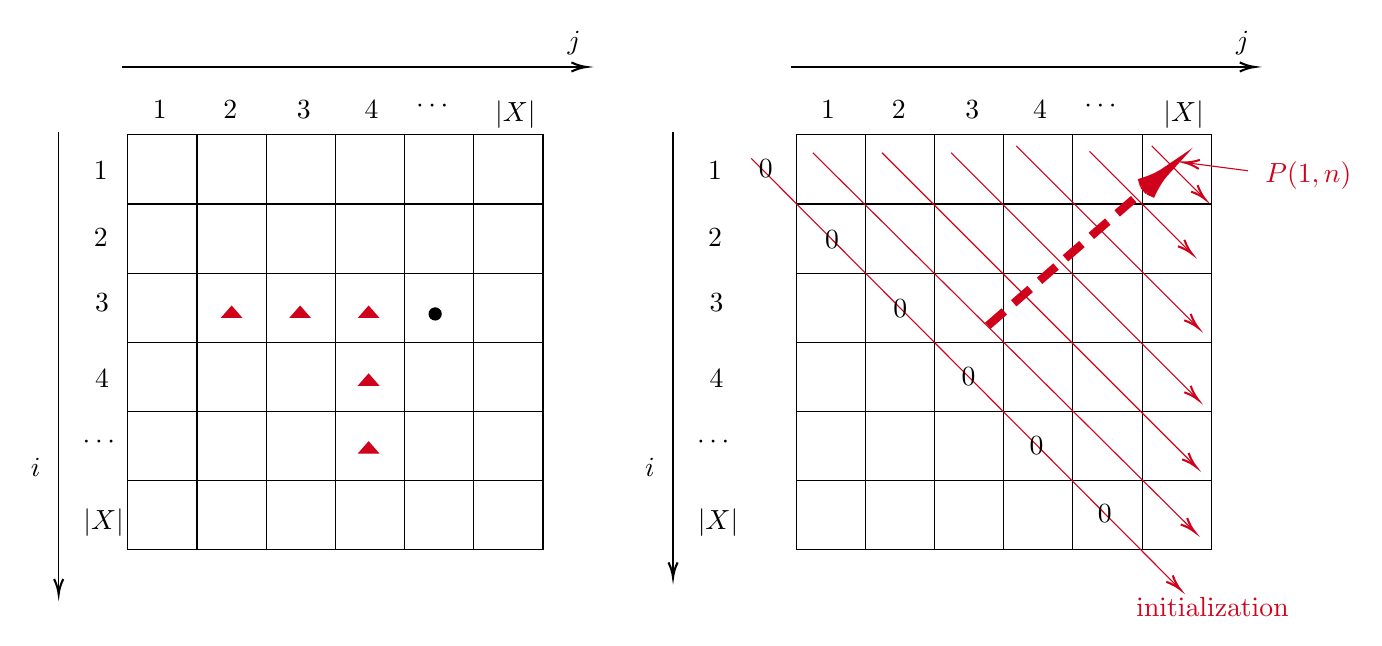
\begin{tikzpicture}[x=0.5pt,y=0.5pt,yscale=-1,xscale=1]
%uncomment if require: \path (0,447); %set diagram left start at 0, and has height of 447

%Shape: Grid [id:dp9095284515127875] 
\draw  [draw opacity=0] (87,90) -- (387,90) -- (387,390) -- (87,390) -- cycle ; \draw   (137,90) -- (137,390)(187,90) -- (187,390)(237,90) -- (237,390)(287,90) -- (287,390)(337,90) -- (337,390) ; \draw   (87,140) -- (387,140)(87,190) -- (387,190)(87,240) -- (387,240)(87,290) -- (387,290)(87,340) -- (387,340) ; \draw   (87,90) -- (387,90) -- (387,390) -- (87,390) -- cycle ;
%Straight Lines [id:da5347307434268296] 
\draw    (37,88) -- (37,420) ;
\draw [shift={(37,422)}, rotate = 270] [color={rgb, 255:red, 0; green, 0; blue, 0 }  ][line width=0.75]    (10.93,-3.29) .. controls (6.95,-1.4) and (3.31,-0.3) .. (0,0) .. controls (3.31,0.3) and (6.95,1.4) .. (10.93,3.29)   ;
%Straight Lines [id:da4989887299865372] 
\draw    (83,41) -- (416.5,41) ;
\draw [shift={(418.5,41)}, rotate = 180] [color={rgb, 255:red, 0; green, 0; blue, 0 }  ][line width=0.75]    (10.93,-3.29) .. controls (6.95,-1.4) and (3.31,-0.3) .. (0,0) .. controls (3.31,0.3) and (6.95,1.4) .. (10.93,3.29)   ;
%Flowchart: Connector [id:dp07878936208838816] 
\draw  [fill={rgb, 255:red, 0; green, 0; blue, 0 }  ,fill opacity=1 ] (305,217.9) .. controls (305.87,215.65) and (308.4,214.52) .. (310.66,215.39) .. controls (312.91,216.26) and (314.04,218.79) .. (313.17,221.05) .. controls (312.3,223.3) and (309.77,224.43) .. (307.51,223.56) .. controls (305.26,222.69) and (304.13,220.16) .. (305,217.9) -- cycle ;
%Shape: Triangle [id:dp6109876057002935] 
\draw  [color={rgb, 255:red, 208; green, 2; blue, 27 }  ,draw opacity=1 ][fill={rgb, 255:red, 208; green, 2; blue, 27 }  ,fill opacity=1 ] (261,214) -- (268,222) -- (254,222) -- cycle ;
%Shape: Triangle [id:dp003677095504452388] 
\draw  [color={rgb, 255:red, 208; green, 2; blue, 27 }  ,draw opacity=1 ][fill={rgb, 255:red, 208; green, 2; blue, 27 }  ,fill opacity=1 ] (211.5,214) -- (218.5,222) -- (204.5,222) -- cycle ;
%Shape: Triangle [id:dp543232883301439] 
\draw  [color={rgb, 255:red, 208; green, 2; blue, 27 }  ,draw opacity=1 ][fill={rgb, 255:red, 208; green, 2; blue, 27 }  ,fill opacity=1 ] (162,214) -- (169,222) -- (155,222) -- cycle ;
%Shape: Triangle [id:dp29900180690969524] 
\draw  [color={rgb, 255:red, 208; green, 2; blue, 27 }  ,draw opacity=1 ][fill={rgb, 255:red, 208; green, 2; blue, 27 }  ,fill opacity=1 ] (261,263) -- (268,271) -- (254,271) -- cycle ;
%Shape: Triangle [id:dp5517868734647194] 
\draw  [color={rgb, 255:red, 208; green, 2; blue, 27 }  ,draw opacity=1 ][fill={rgb, 255:red, 208; green, 2; blue, 27 }  ,fill opacity=1 ] (261,312) -- (268,320) -- (254,320) -- cycle ;
%Shape: Grid [id:dp8676217076414684] 
\draw  [draw opacity=0] (570,90) -- (870,90) -- (870,390) -- (570,390) -- cycle ; \draw   (620,90) -- (620,390)(670,90) -- (670,390)(720,90) -- (720,390)(770,90) -- (770,390)(820,90) -- (820,390) ; \draw   (570,140) -- (870,140)(570,190) -- (870,190)(570,240) -- (870,240)(570,290) -- (870,290)(570,340) -- (870,340) ; \draw   (570,90) -- (870,90) -- (870,390) -- (570,390) -- cycle ;
%Straight Lines [id:da23917339503157053] 
\draw    (481,88) -- (481,408) ;
\draw [shift={(481,410)}, rotate = 270] [color={rgb, 255:red, 0; green, 0; blue, 0 }  ][line width=0.75]    (10.93,-3.29) .. controls (6.95,-1.4) and (3.31,-0.3) .. (0,0) .. controls (3.31,0.3) and (6.95,1.4) .. (10.93,3.29)   ;
%Straight Lines [id:da1200250503088851] 
\draw    (566,41) -- (899.5,41) ;
\draw [shift={(901.5,41)}, rotate = 180] [color={rgb, 255:red, 0; green, 0; blue, 0 }  ][line width=0.75]    (10.93,-3.29) .. controls (6.95,-1.4) and (3.31,-0.3) .. (0,0) .. controls (3.31,0.3) and (6.95,1.4) .. (10.93,3.29)   ;
%Straight Lines [id:da5849775638339646] 
\draw [color={rgb, 255:red, 208; green, 2; blue, 27 }  ,draw opacity=1 ]   (896.5,116) -- (852.48,110.26) ;
\draw [shift={(850.5,110)}, rotate = 367.43] [color={rgb, 255:red, 208; green, 2; blue, 27 }  ,draw opacity=1 ][line width=0.75]    (10.93,-3.29) .. controls (6.95,-1.4) and (3.31,-0.3) .. (0,0) .. controls (3.31,0.3) and (6.95,1.4) .. (10.93,3.29)   ;
%Straight Lines [id:da7158674315801672] 
\draw [color={rgb, 255:red, 208; green, 2; blue, 27 }  ,draw opacity=1 ]   (537.5,107) -- (846.09,417.08) ;
\draw [shift={(847.5,418.5)}, rotate = 225.14] [color={rgb, 255:red, 208; green, 2; blue, 27 }  ,draw opacity=1 ][line width=0.75]    (10.93,-3.29) .. controls (6.95,-1.4) and (3.31,-0.3) .. (0,0) .. controls (3.31,0.3) and (6.95,1.4) .. (10.93,3.29)   ;
%Straight Lines [id:da06318163354731099] 
\draw [color={rgb, 255:red, 208; green, 2; blue, 27 }  ,draw opacity=1 ]   (582,103) -- (856.58,375.59) ;
\draw [shift={(858,377)}, rotate = 224.79] [color={rgb, 255:red, 208; green, 2; blue, 27 }  ,draw opacity=1 ][line width=0.75]    (10.93,-3.29) .. controls (6.95,-1.4) and (3.31,-0.3) .. (0,0) .. controls (3.31,0.3) and (6.95,1.4) .. (10.93,3.29)   ;
%Straight Lines [id:da7422545951430948] 
\draw [color={rgb, 255:red, 208; green, 2; blue, 27 }  ,draw opacity=1 ]   (632,103) -- (857.59,328.59) ;
\draw [shift={(859,330)}, rotate = 225] [color={rgb, 255:red, 208; green, 2; blue, 27 }  ,draw opacity=1 ][line width=0.75]    (10.93,-3.29) .. controls (6.95,-1.4) and (3.31,-0.3) .. (0,0) .. controls (3.31,0.3) and (6.95,1.4) .. (10.93,3.29)   ;
%Straight Lines [id:da6389984033381221] 
\draw [color={rgb, 255:red, 208; green, 2; blue, 27 }  ,draw opacity=1 ]   (682,103) -- (859.09,280.09) ;
\draw [shift={(860.5,281.5)}, rotate = 225] [color={rgb, 255:red, 208; green, 2; blue, 27 }  ,draw opacity=1 ][line width=0.75]    (10.93,-3.29) .. controls (6.95,-1.4) and (3.31,-0.3) .. (0,0) .. controls (3.31,0.3) and (6.95,1.4) .. (10.93,3.29)   ;
%Straight Lines [id:da7613617756284687] 
\draw [color={rgb, 255:red, 208; green, 2; blue, 27 }  ,draw opacity=1 ]   (729,98) -- (859.09,228.09) ;
\draw [shift={(860.5,229.5)}, rotate = 225] [color={rgb, 255:red, 208; green, 2; blue, 27 }  ,draw opacity=1 ][line width=0.75]    (10.93,-3.29) .. controls (6.95,-1.4) and (3.31,-0.3) .. (0,0) .. controls (3.31,0.3) and (6.95,1.4) .. (10.93,3.29)   ;
%Straight Lines [id:da7035765059521567] 
\draw [color={rgb, 255:red, 208; green, 2; blue, 27 }  ,draw opacity=1 ]   (782,102) -- (854.59,174.59) ;
\draw [shift={(856,176)}, rotate = 225] [color={rgb, 255:red, 208; green, 2; blue, 27 }  ,draw opacity=1 ][line width=0.75]    (10.93,-3.29) .. controls (6.95,-1.4) and (3.31,-0.3) .. (0,0) .. controls (3.31,0.3) and (6.95,1.4) .. (10.93,3.29)   ;
%Straight Lines [id:da156242521236438] 
\draw [color={rgb, 255:red, 208; green, 2; blue, 27 }  ,draw opacity=1 ]   (827,98) -- (864.09,135.09) ;
\draw [shift={(865.5,136.5)}, rotate = 225] [color={rgb, 255:red, 208; green, 2; blue, 27 }  ,draw opacity=1 ][line width=0.75]    (10.93,-3.29) .. controls (6.95,-1.4) and (3.31,-0.3) .. (0,0) .. controls (3.31,0.3) and (6.95,1.4) .. (10.93,3.29)   ;
%Straight Lines [id:da421849353700268] 
\draw [color={rgb, 255:red, 208; green, 2; blue, 27 }  ,draw opacity=1 ][line width=3]  [dash pattern={on 7.88pt off 4.5pt}]  (708.5,228) -- (833.72,119.28) ;
\draw [shift={(837.5,116)}, rotate = 499.03] [color={rgb, 255:red, 208; green, 2; blue, 27 }  ,draw opacity=1 ][line width=3]    (20.77,-6.25) .. controls (13.2,-2.65) and (6.28,-0.57) .. (0,0) .. controls (6.28,0.57) and (13.2,2.66) .. (20.77,6.25)   ;

% Text Node
\draw (68,103) node [anchor=north west][inner sep=0.75pt]   [align=left] {$ $};
% Text Node
\draw (60.5,107.38) node [anchor=north west][inner sep=0.75pt]   [align=left] {$\displaystyle 1$};
% Text Node
\draw (52.5,306.14) node [anchor=north west][inner sep=0.75pt]   [align=left] {$\displaystyle \cdots $};
% Text Node
\draw (15,322) node [anchor=north west][inner sep=0.75pt]   [align=left] {$\displaystyle i$};
% Text Node
\draw (403,13) node [anchor=north west][inner sep=0.75pt]   [align=left] {$\displaystyle j$};
% Text Node
\draw (293.4,63.44) node [anchor=north west][inner sep=0.75pt]   [align=left] {$\displaystyle \cdots $};
% Text Node
\draw (60.5,155.76) node [anchor=north west][inner sep=0.75pt]   [align=left] {$\displaystyle 2$};
% Text Node
\draw (103.1,63.44) node [anchor=north west][inner sep=0.75pt]   [align=left] {$\displaystyle 1$};
% Text Node
\draw (154.2,63.44) node [anchor=north west][inner sep=0.75pt]   [align=left] {$\displaystyle 2$};
% Text Node
\draw (350.5,63.44) node [anchor=north west][inner sep=0.75pt]   [align=left] {$\displaystyle | X|$};
% Text Node
\draw (207.3,63.44) node [anchor=north west][inner sep=0.75pt]   [align=left] {$\displaystyle 3$};
% Text Node
\draw (53,358.5) node [anchor=north west][inner sep=0.75pt]   [align=left] {$\displaystyle | X|$};
% Text Node
\draw (61.5,202.76) node [anchor=north west][inner sep=0.75pt]   [align=left] {$\displaystyle 3$};
% Text Node
\draw (61.5,257.76) node [anchor=north west][inner sep=0.75pt]   [align=left] {$\displaystyle 4$};
% Text Node
\draw (256.3,63.44) node [anchor=north west][inner sep=0.75pt]   [align=left] {$\displaystyle 4$};
% Text Node
\draw (512,103) node [anchor=north west][inner sep=0.75pt]   [align=left] {$ $};
% Text Node
\draw (504.5,107.38) node [anchor=north west][inner sep=0.75pt]   [align=left] {$\displaystyle 1$};
% Text Node
\draw (496.5,306.14) node [anchor=north west][inner sep=0.75pt]   [align=left] {$\displaystyle \cdots $};
% Text Node
\draw (459,322) node [anchor=north west][inner sep=0.75pt]   [align=left] {$\displaystyle i$};
% Text Node
\draw (886,13) node [anchor=north west][inner sep=0.75pt]   [align=left] {$\displaystyle j$};
% Text Node
\draw (776.4,63.44) node [anchor=north west][inner sep=0.75pt]   [align=left] {$\displaystyle \cdots $};
% Text Node
\draw (504.5,155.76) node [anchor=north west][inner sep=0.75pt]   [align=left] {$\displaystyle 2$};
% Text Node
\draw (586.1,63.44) node [anchor=north west][inner sep=0.75pt]   [align=left] {$\displaystyle 1$};
% Text Node
\draw (637.2,63.44) node [anchor=north west][inner sep=0.75pt]   [align=left] {$\displaystyle 2$};
% Text Node
\draw (833.5,63.44) node [anchor=north west][inner sep=0.75pt]   [align=left] {$\displaystyle | X|$};
% Text Node
\draw (690.3,63.44) node [anchor=north west][inner sep=0.75pt]   [align=left] {$\displaystyle 3$};
% Text Node
\draw (907.2,107.44) node [anchor=north west][inner sep=0.75pt]   [align=left] {$\displaystyle \textcolor[rgb]{0.82,0.01,0.11}{P}\textcolor[rgb]{0.82,0.01,0.11}{(}\textcolor[rgb]{0.82,0.01,0.11}{1,n}\textcolor[rgb]{0.82,0.01,0.11}{)}$};
% Text Node
\draw (497,358.5) node [anchor=north west][inner sep=0.75pt]   [align=left] {$\displaystyle | X|$};
% Text Node
\draw (505.5,202.76) node [anchor=north west][inner sep=0.75pt]   [align=left] {$\displaystyle 3$};
% Text Node
\draw (505.5,257.76) node [anchor=north west][inner sep=0.75pt]   [align=left] {$\displaystyle 4$};
% Text Node
\draw (739.3,63.44) node [anchor=north west][inner sep=0.75pt]   [align=left] {$\displaystyle 4$};
% Text Node
\draw (589.1,157.44) node [anchor=north west][inner sep=0.75pt]   [align=left] {$\displaystyle 0$};
% Text Node
\draw (638.35,206.94) node [anchor=north west][inner sep=0.75pt]   [align=left] {$\displaystyle 0$};
% Text Node
\draw (687.6,256.44) node [anchor=north west][inner sep=0.75pt]   [align=left] {$\displaystyle 0$};
% Text Node
\draw (736.85,305.94) node [anchor=north west][inner sep=0.75pt]   [align=left] {$\displaystyle 0$};
% Text Node
\draw (786.1,355.44) node [anchor=north west][inner sep=0.75pt]   [align=left] {$\displaystyle 0$};
% Text Node
\draw (814,422) node [anchor=north west][inner sep=0.75pt]   [align=left] {\textcolor[rgb]{0.82,0.01,0.11}{initialization}};
% Text Node
\draw (541.1,106.44) node [anchor=north west][inner sep=0.75pt]   [align=left] {$\displaystyle 0$};


\end{tikzpicture}

}
\caption{Illustration of the dynamic programming table for shortest-path problem.}
\label{fig:table}
\end{figure}


A typical dynamic programming algorithm can be organized into 3 steps.
The \emph{initialization step}, in this case, fills the first row of the table:
$dist(0,s) = 0$ and $dist(0,v) = \infty$ if $v\neq s$.
The \emph{iteration step} fills all other rows of the table using above recursion.
The \emph{termination step} answers the original question, in this case,
reports that the last row gives the distance for every vertex.
The pseudo-code is given below.
Try run this algorithm~(fill the dynamic programming table) on the example below.

\begin{minipage}{0.8\textwidth}
	\aaA {14}{Algorithm DP-shortest-path~($G = (V, E)$, $l(e)$ for any $e\in E$, $s \in V$)}\xxx
	\aab {init a 2D array $dist$ of size $|V|\times |V|$;}\xxx
	\aab {$dist[0, s] = 0$; $dist[0, v] = \infty$ for any $v\neq s$;}\xxx
	\aaB {9}{for $k = 1 \to |V| - 1$;}\xxx
	\aaC {7}{for $v\in V$;}\xxx
	\aad {$dist(k,v) = dist(k-1, v)$;}\xxx
	\aaD {4}{for each $(u,v)\in E$;}\xxx
	\aaE {2}{if~($dist(k,v) > dist(k-1,u) + l(u,v)$)}\xxx
	\aaf {$dist(k,v) = dist(k-1,u) + l(u,v)$;}\xxx
	\aae {end if;}\xxx
	\aad {end for;}\xxx
	\aac {end for;}\xxx
	\aab {end for;}\xxx
	\aab {$dist[|V|-1,v]$ gives $distance(s,v)$, for any $v\in V$;}\xxx
	\aaa {end algorithm;}\xxx
\end{minipage}

\begin{figure}[h]
\centering{

\tikzset{every picture/.style={line width=0.75pt}} %set default line width to 0.75pt        

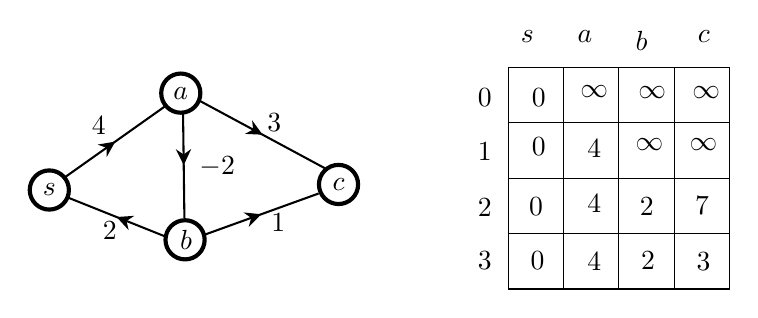
\begin{tikzpicture}[x=0.5pt,y=0.5pt,yscale=-1,xscale=1]
%uncomment if require: \path (0,223); %set diagram left start at 0, and has height of 223

%Shape: Grid [id:dp8546141469296037] 
\draw  [draw opacity=0] (364,36) -- (524,36) -- (524,196) -- (364,196) -- cycle ; \draw   (404,36) -- (404,196)(444,36) -- (444,196)(484,36) -- (484,196) ; \draw   (364,76) -- (524,76)(364,116) -- (524,116)(364,156) -- (524,156) ; \draw   (364,36) -- (524,36) -- (524,196) -- (364,196) -- cycle ;
%Straight Lines [id:da47377092575328894] 
\draw [color={rgb, 255:red, 0; green, 0; blue, 0 }  ,draw opacity=1 ][line width=0.75]    (44,115) -- (116,64) ;
\draw [shift={(80,89.5)}, rotate = 504.69] [fill={rgb, 255:red, 0; green, 0; blue, 0 }  ,fill opacity=1 ][line width=0.08]  [draw opacity=0] (11.61,-5.58) -- (0,0) -- (11.61,5.58) -- (7.71,0) -- cycle    ;
%Straight Lines [id:da6214062451740884] 
\draw [color={rgb, 255:red, 0; green, 0; blue, 0 }  ,draw opacity=1 ][line width=0.75]    (46,130) -- (116,158) ;
\draw [shift={(81,144)}, rotate = 21.8] [fill={rgb, 255:red, 0; green, 0; blue, 0 }  ,fill opacity=1 ][line width=0.08]  [draw opacity=0] (11.61,-5.58) -- (0,0) -- (11.61,5.58) -- (7.71,0) -- cycle    ;
%Straight Lines [id:da8467518623200763] 
\draw [color={rgb, 255:red, 0; green, 0; blue, 0 }  ,draw opacity=1 ][line width=0.75]    (227,127) -- (144,157) ;
\draw [shift={(185.5,142)}, rotate = 160.13] [fill={rgb, 255:red, 0; green, 0; blue, 0 }  ,fill opacity=1 ][line width=0.08]  [draw opacity=0] (11.61,-5.58) -- (0,0) -- (11.61,5.58) -- (7.71,0) -- cycle    ;
%Straight Lines [id:da524270381396472] 
\draw [color={rgb, 255:red, 0; green, 0; blue, 0 }  ,draw opacity=1 ][line width=0.75]    (232,109) -- (141,60) ;
\draw [shift={(186.5,84.5)}, rotate = 208.3] [fill={rgb, 255:red, 0; green, 0; blue, 0 }  ,fill opacity=1 ][line width=0.08]  [draw opacity=0] (11.61,-5.58) -- (0,0) -- (11.61,5.58) -- (7.71,0) -- cycle    ;
%Straight Lines [id:da24886819030904006] 
\draw [color={rgb, 255:red, 0; green, 0; blue, 0 }  ,draw opacity=1 ][line width=0.75]    (129,68) -- (130,145) ;
\draw [shift={(129.5,106.5)}, rotate = 269.26] [fill={rgb, 255:red, 0; green, 0; blue, 0 }  ,fill opacity=1 ][line width=0.08]  [draw opacity=0] (11.61,-5.58) -- (0,0) -- (11.61,5.58) -- (7.71,0) -- cycle    ;

% Text Node
\draw (379.24,49.06) node [anchor=north west][inner sep=0.75pt]   [align=left] {$\displaystyle 0$};
% Text Node
\draw (340.24,88.56) node [anchor=north west][inner sep=0.75pt]   [align=left] {$\displaystyle 1$};
% Text Node
\draw (340.24,129.06) node [anchor=north west][inner sep=0.75pt]   [align=left] {$\displaystyle 2$};
% Text Node
\draw (371.24,7.56) node [anchor=north west][inner sep=0.75pt]   [align=left] {$\displaystyle s$};
% Text Node
\draw (412.24,7.56) node [anchor=north west][inner sep=0.75pt]   [align=left] {$\displaystyle a$};
% Text Node
\draw (454.24,7.56) node [anchor=north west][inner sep=0.75pt]   [align=left] {$\displaystyle b$};
% Text Node
\draw (499.24,7.56) node [anchor=north west][inner sep=0.75pt]   [align=left] {$\displaystyle c$};
% Text Node
\draw (414.24,47.06) node [anchor=north west][inner sep=0.75pt]   [align=left] {$\displaystyle \infty $};
% Text Node
\draw (456.24,48.06) node [anchor=north west][inner sep=0.75pt]   [align=left] {$\displaystyle \infty $};
% Text Node
\draw (495.24,48.06) node [anchor=north west][inner sep=0.75pt]   [align=left] {$\displaystyle \infty $};
% Text Node
\draw (340.24,49.06) node [anchor=north west][inner sep=0.75pt]   [align=left] {$\displaystyle 0$};
% Text Node
\draw (340.24,167.06) node [anchor=north west][inner sep=0.75pt]   [align=left] {$\displaystyle 3$};
% Text Node
\draw (493.24,85.06) node [anchor=north west][inner sep=0.75pt]   [align=left] {$\displaystyle \infty $};
% Text Node
\draw (454.24,85.06) node [anchor=north west][inner sep=0.75pt]   [align=left] {$\displaystyle \infty $};
% Text Node
\draw (379.24,85.06) node [anchor=north west][inner sep=0.75pt]   [align=left] {$\displaystyle 0$};
% Text Node
\draw (419.24,86.06) node [anchor=north west][inner sep=0.75pt]   [align=left] {$\displaystyle 4$};
% Text Node
\draw (419.24,126.06) node [anchor=north west][inner sep=0.75pt]   [align=left] {$\displaystyle 4$};
% Text Node
\draw (419.24,168.06) node [anchor=north west][inner sep=0.75pt]   [align=left] {$\displaystyle 4$};
% Text Node
\draw (377.24,128.06) node [anchor=north west][inner sep=0.75pt]   [align=left] {$\displaystyle 0$};
% Text Node
\draw (378.24,167.06) node [anchor=north west][inner sep=0.75pt]   [align=left] {$\displaystyle 0$};
% Text Node
\draw (457.24,128.06) node [anchor=north west][inner sep=0.75pt]   [align=left] {$\displaystyle 2$};
% Text Node
\draw (458.24,167.06) node [anchor=north west][inner sep=0.75pt]   [align=left] {$\displaystyle 2$};
% Text Node
\draw (498.24,168.06) node [anchor=north west][inner sep=0.75pt]   [align=left] {$\displaystyle 3$};
% Text Node
\draw (497.24,127.06) node [anchor=north west][inner sep=0.75pt]   [align=left] {$\displaystyle 7$};
% Text Node
\draw (69.24,145.53) node [anchor=north west][inner sep=0.75pt]   [align=left] {$\displaystyle 2$};
% Text Node
\draw  [line width=1.5]   (32.38, 124.47) circle [x radius= 14.15, y radius= 14.15]   ;
\draw (32.38,124.47) node   [align=left] {$\displaystyle s$};
% Text Node
\draw  [line width=1.5]   (127.38, 54.47) circle [x radius= 14.15, y radius= 14.15]   ;
\draw (127.38,54.47) node   [align=left] {$\displaystyle a$};
% Text Node
\draw  [line width=1.5]   (130.48, 160.47) circle [x radius= 14.15, y radius= 14.15]   ;
\draw (124.98,160.47) node [anchor=west] [inner sep=0.75pt]   [align=left] {$\displaystyle b$};
% Text Node
\draw  [line width=1.5]   (241.38, 120.47) circle [x radius= 14.15, y radius= 14.15]   ;
\draw (241.38,120.47) node   [align=left] {$\displaystyle c$};
% Text Node
\draw (61.24,69.53) node [anchor=north west][inner sep=0.75pt]   [align=left] {$\displaystyle 4$};
% Text Node
\draw (188,67.47) node [anchor=north west][inner sep=0.75pt]   [align=left] {$\displaystyle 3$};
% Text Node
\draw (191,139.47) node [anchor=north west][inner sep=0.75pt]   [align=left] {$\displaystyle 1$};
% Text Node
\draw (139,98.47) node [anchor=north west][inner sep=0.75pt]   [align=left] {$\displaystyle -2$};


\end{tikzpicture}

}
\caption{An example of running above DP algorithm.}
\label{fig:table}
\end{figure}


The second for-loop and the the third for-loop together take $O(|E|)$ time,
as it examines, for each $v\in V$, the in-edges of $v$.
Hence, the running time of this algorithm is $O(|V|\cdot |E|)$.

\subsection*{Recursion Revisited}

In the core recursion of the DP algorithm,
$dist(k,\cdot)$ only depends on $dist(k - 1, \cdot)$.
In other words, the calculation of next row of the DP table
only relies on the value of the previous row.
This property has the following two applications.

{\bf Early Termination.} In any run of the DP algorithm, if we observe
that the $k$-th row and $(k+1)$-th row are identical,
then the algorithm can be terminated~(rather than keep running it until the $(|V|-1)$-th row),
as we know that any of the future row will be identical to these two rows.

{\bf Space Complexity.} It seems that the DP algorithm requires $|V|^2$ space,
as the DP table is $|V|\times |V|$.
In fact, this can be improved to $2|V|$,
as we only need to maintain two rows, the current row and
the previous row; the completion of the current row uses the values 
in the previous row, and after the current row has been completed,
copy it to the previous row.

\subsection*{Characterization of Negative Cycle}

We focus on this problem: given graph $G = (V,E)$ with edge length $l(e)$, $e\in E$, and
a source vertex $s$, to decide if there exists a negative cycle in $G$ that is reachable from $s$.
Before we design algorithm for it,
we first derive an equivalent characterization.

Recall that $dist(k,v)$ is defined as the length of the shortest path from $s$ to $v$ using
at most $k$ edges. We emphasize that, this definition is still valid in the presence of negative cycles.
Comparing with $distance(s,v)$, which may not be well-defined as the shortest path may use unlimited
number of edges, the definition of $dist(k,v)$ limits the number of edges~(i.e., $k$) in the path.
Hence, $dist(k,v)$ is well-defined for any $k\ge 0$ and any $v\in V$. See an example below.

\begin{figure}[h]
\centering{

\tikzset{every picture/.style={line width=0.75pt}} %set default line width to 0.75pt        

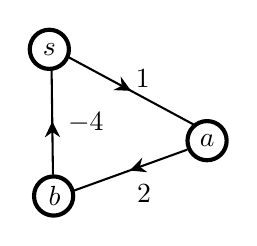
\begin{tikzpicture}[x=0.5pt,y=0.5pt,yscale=-1,xscale=1]
%uncomment if require: \path (0,174); %set diagram left start at 0, and has height of 174

%Straight Lines [id:da6034488908673977] 
\draw [color={rgb, 255:red, 0; green, 0; blue, 0 }  ,draw opacity=1 ][line width=0.75]    (146,105) -- (63,135) ;
\draw [shift={(104.5,120)}, rotate = 340.13] [fill={rgb, 255:red, 0; green, 0; blue, 0 }  ,fill opacity=1 ][line width=0.08]  [draw opacity=0] (11.61,-5.58) -- (0,0) -- (11.61,5.58) -- (7.71,0) -- cycle    ;
%Straight Lines [id:da5375746664082175] 
\draw [color={rgb, 255:red, 0; green, 0; blue, 0 }  ,draw opacity=1 ][line width=0.75]    (151,87) -- (60,38) ;
\draw [shift={(105.5,62.5)}, rotate = 208.3] [fill={rgb, 255:red, 0; green, 0; blue, 0 }  ,fill opacity=1 ][line width=0.08]  [draw opacity=0] (11.61,-5.58) -- (0,0) -- (11.61,5.58) -- (7.71,0) -- cycle    ;
%Straight Lines [id:da43457397683408727] 
\draw [color={rgb, 255:red, 0; green, 0; blue, 0 }  ,draw opacity=1 ][line width=0.75]    (48,46) -- (49,123) ;
\draw [shift={(48.5,84.5)}, rotate = 89.26] [fill={rgb, 255:red, 0; green, 0; blue, 0 }  ,fill opacity=1 ][line width=0.08]  [draw opacity=0] (11.61,-5.58) -- (0,0) -- (11.61,5.58) -- (7.71,0) -- cycle    ;

% Text Node
\draw  [line width=1.5]   (46.38, 32.47) circle [x radius= 14.15, y radius= 14.15]   ;
\draw (46.38,32.47) node   [align=left] {$\displaystyle s$};
% Text Node
\draw  [line width=1.5]   (49.48, 138.47) circle [x radius= 14.15, y radius= 14.15]   ;
\draw (43.98,138.47) node [anchor=west] [inner sep=0.75pt]   [align=left] {$\displaystyle b$};
% Text Node
\draw  [line width=1.5]   (160.38, 98.47) circle [x radius= 14.15, y radius= 14.15]   ;
\draw (160.38,98.47) node   [align=left] {$\displaystyle a$};
% Text Node
\draw (107,45.47) node [anchor=north west][inner sep=0.75pt]   [align=left] {$\displaystyle 1$};
% Text Node
\draw (108,128.47) node [anchor=north west][inner sep=0.75pt]   [align=left] {$\displaystyle 2$};
% Text Node
\draw (58,76.47) node [anchor=north west][inner sep=0.75pt]   [align=left] {$\displaystyle -4$};


\end{tikzpicture}

}
\caption{Example showing that $dist(k,v)$ is well-defined in the presence of negative cycle.
In this example, $dist(1,a) = 1$, $dist(301,a) = -99$, $dist(3001,a) = -999$.}
\label{fig:space}
\end{figure}

\begin{fact}
Let $C$ be a negative cycle reachable from $s$;
let $v\in C$. Then we have $\lim_{k\to\infty} dist(k,v) = -\infty$.
\end{fact}
\emph{Proof.} This is because, one can loop within $C$ to get shorter and shorter path from $s$ to $v$. \qed

%On the other hand, if $C$ does not contain negative cycle, then $dist(|V| - 1, v) = distance(s,v)$.
%Note that $dist(k + 1, v) \le dist(k, v)$, for any $k\ge 0$, as $dist(k+1,v)$ is the optimal solution of a larger sub-space than that of $dist(k,v)$.
%Note that too $dist(k,v) \ge distance(s,v)$, for any $k\ge 0$, again because $distance(s,v)$ is the optimal solution of the entire search space~(and
%$distance(s,v)$ is well-defined without negative cycle).
%This leads to that, if $G$ does not contain cycle, when $k\ge |V| - 1$, we always have 
%$dist(k, v) = dist(|V| - 1, v) = distance(s,v)$.
%
%Combined, we have the following chracterization of the existence of negative cycle reachable from $s$.
%\begin{claim}
%A graph $G$ contains a negative cycle reachable from $s$ if and only if there exists a vertex $v$ such that
%$\lim_{k\to\infty} dist(k,v) = -\infty$.
%\end{claim}

\subsection*{DP Algorithm to Detect Negative Cycle}

We will extend above DP algorithm to do it.
Recall that the DP consists of initialization, iteration, and termination steps.
We emphasize that, in the presence of negative cycles, the initialization and iteration
steps are still correct~(simply because the proof of their correctness doesn't assume that $G$ does not contain negative cycle),
i.e., we can still use them to calculate $dist(k,v)$, for \emph{any} $k\ge 0$, even if $G$ contains negative cycle.
It's only that the termination step won't work in the presence of neagive cycle,
as $dist(|V| - 1, v) = distance(s,v)$ needs the condition that $G$ does not contain negative cycle.
Note too that the early-termination property is also correct in the presence of negative cycles.

Here comes the algorithm to decide negative cycle reachable from $s$:
it simply calculates one more row in the DP table and check if the last two rows are identical.

\begin{minipage}{0.8\textwidth}
	\aaA {7}{Algorithm detect-negagive-cycle~($G = (V, E)$, $l(e)$ for any $e\in E$, $s \in V$)}\xxx
	\aab {fill one more row in the DP table, i.e., calculate $dist(|V|, v)$ for any $v\in V$;}\xxx
	\aaB {2}{if~($dist(|V|,v) = dist(|V| - 1,v)$ for \emph{every} $v\in V$)}\xxx
	\aac {report: ``$G$ does not contain negative cycle reachable from $s$'';}\xxx
	\aaB {2}{else}\xxx
	\aac {report: ``$G$ contains negative cycle reachable from $s$'';}\xxx
	\aab {end if;}\xxx
	\aaa {end algorithm;}\xxx
\end{minipage}

We now prove the correctness of the above algorithm.
The proof is a combination of the facts we have seen, namely Fact~1 in Lecture~19, the ``early-termination'' property,
and Fact~1 in this lecture.

\emph{Proof.} We first prove that, if $G$ does not contain negaive cycle reachable from $s$, then $dist(|V|, v) = dist(|V| - 1, v)$ for every $v\in V$.
Following Fact~1 in Lecture~19, we have $dist(|V| - 1, v) = distance(s,v)$.
Note that $dist(|V|, v) \le dist(|V| - 1, v)$, as $dist(|V|,v)$ is the optimal solution of a larger sub-space than that of $dist(|V|-1,v)$.
Note too that $dist(|V|,v) \ge distance(s,v)$, as $distance(s,v)$ is the optimal solution of the entire search space~(and
$distance(s,v)$ is well-defined without negative cycle).
Combined, $dist(|V|, v) = dist(|V| - 1, v)$ for every $v\in V$.

We then prove that, if $G$ contains negaive cycle reachable from $s$, then there exist $v\in V$ such that $dist(|V|, v) \neq dist(|V| - 1, v)$.
Suppose conversely that $dist(|V|, v) = dist(|V| - 1, v)$ for every $v\in V$.
Then following the early-termination property, any future row will be the same as $dist(|V|-1,v)$, i.e., $\lim_{k\to\infty} dist(k, v) = dist(|V| - 1, v)$, for every $v\in V$.
This contradicts to the Fact~1 in this lecture. \qed

\subsection*{Floyd-Warshall Algorithm}

We consider the \emph{all-pairs shortest path problem}: given graph $G = (V, E)$ with edge length $l(e)$ for any $e\in E$,
to compute $distance(u,v)$ for any $u,v\in V$. A straitforward algorithm is to run any algorithm for single-source shortest path problem
$|V|$ times, in each of which starting from a different vertex as source. The running time will be $O(|V|^2|E|)$.

We now introduce Floyd-Warshall algorithm, which takes $O(|V|^3)$ time.
Instead of limiting the number of edges in the shortest paths as used in the DP algorithms for single-source shortest path problem,
in Floyd-Warshall algorithm, we limit the \emph{largest index of the intermediate vertices} in the shortest paths.
Specifically, we rename $V = \{v_1, v_2, \cdots, v_n\}$, where $n = |V|$.
We define $dist(i,j,k)$ as the length of the shortest path from $v_i$ to $v_j$
such that the intermediate vertices on the path is from $\{v_1, v_2, \cdots, v_k\}$.
In other words, among all paths from $v_i$ to $v_j$ with 
intermediate vertices being from $\{v_1, v_2, \cdots, v_k\}$,
$dist(i,j,k)$ gives the length of the shortest one.
Clearly, we have that $distance(v_i, v_j) = dist(i, j, n)$.

Now let's develop a recursion.
Let $p$ be the shortest path from $v_i$ to $v_j$ with 
intermediate vertices being from $\{v_1, v_2, \cdots, v_k\}$.
There are two possibilities: $p$ does not use $v_k$ and $p$ uses $v_k$.
If it is the first case, we know that $dist(i,j,k) = dist(i,j,k-1)$.
If it is the second case, $p$ is partitioned into two paths, one from $v_i$ to $v_k$ and the other is from $v_k$ to $v_j$,
and in either path the 
intermediate vertices must be from $\{v_1, v_2, \cdots, v_{k-1}\}$.
Therefore, in this case, $dist(i,j,k) = dist(i,k,k-1) + dist(k,j,k-1)$.
Combined, we have the following recursion:
$$dist(i,j,k) = \min\{dist(i,j,k-1), dist(i,k,k-1) + dist(k,j,k-1)\}.$$

\begin{figure}[h]
\centering{

\tikzset{every picture/.style={line width=0.75pt}} %set default line width to 0.75pt        

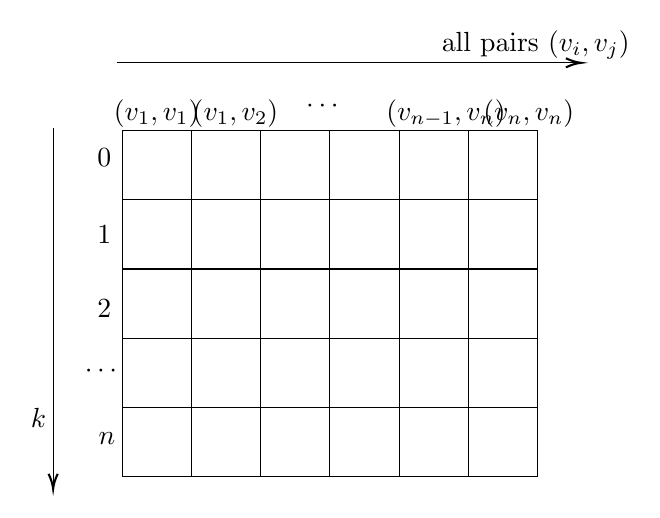
\begin{tikzpicture}[x=0.5pt,y=0.5pt,yscale=-1,xscale=1]
%uncomment if require: \path (0,370); %set diagram left start at 0, and has height of 370

%Shape: Grid [id:dp9095284515127875] 
\draw  [draw opacity=0] (87,90) -- (387,90) -- (387,340) -- (87,340) -- cycle ; \draw   (137,90) -- (137,340)(187,90) -- (187,340)(237,90) -- (237,340)(287,90) -- (287,340)(337,90) -- (337,340) ; \draw   (87,140) -- (387,140)(87,190) -- (387,190)(87,240) -- (387,240)(87,290) -- (387,290) ; \draw   (87,90) -- (387,90) -- (387,340) -- (87,340) -- cycle ;
%Straight Lines [id:da5347307434268296] 
\draw    (37,88) -- (37,347) ;
\draw [shift={(37,349)}, rotate = 270] [color={rgb, 255:red, 0; green, 0; blue, 0 }  ][line width=0.75]    (10.93,-3.29) .. controls (6.95,-1.4) and (3.31,-0.3) .. (0,0) .. controls (3.31,0.3) and (6.95,1.4) .. (10.93,3.29)   ;
%Straight Lines [id:da4989887299865372] 
\draw    (83,41) -- (416.5,41) ;
\draw [shift={(418.5,41)}, rotate = 180] [color={rgb, 255:red, 0; green, 0; blue, 0 }  ][line width=0.75]    (10.93,-3.29) .. controls (6.95,-1.4) and (3.31,-0.3) .. (0,0) .. controls (3.31,0.3) and (6.95,1.4) .. (10.93,3.29)   ;

% Text Node
\draw (67,101) node [anchor=north west][inner sep=0.75pt]   [align=left] {$\displaystyle 0$};
% Text Node
\draw (67,156.5) node [anchor=north west][inner sep=0.75pt]   [align=left] {$\displaystyle 1$};
% Text Node
\draw (67,210) node [anchor=north west][inner sep=0.75pt]   [align=left] {$\displaystyle 2$};
% Text Node
\draw (58,257.5) node [anchor=north west][inner sep=0.75pt]   [align=left] {$\displaystyle \cdots $};
% Text Node
\draw (68,306) node [anchor=north west][inner sep=0.75pt]   [align=left] {$\displaystyle n$};
% Text Node
\draw (19,289) node [anchor=north west][inner sep=0.75pt]   [align=left] {$\displaystyle k$};
% Text Node
\draw (316,16) node [anchor=north west][inner sep=0.75pt]   [align=left] {all pairs $\displaystyle ( v_{i} ,v_{j})$};
% Text Node
\draw (79,66) node [anchor=north west][inner sep=0.75pt]   [align=left] {$\displaystyle ( v_{1} ,v_{1})$};
% Text Node
\draw (346,66) node [anchor=north west][inner sep=0.75pt]   [align=left] {$\displaystyle ( v_{n} ,v_{n})$};
% Text Node
\draw (136,66) node [anchor=north west][inner sep=0.75pt]   [align=left] {$\displaystyle ( v_{1} ,v_{2})$};
% Text Node
\draw (218,66) node [anchor=north west][inner sep=0.75pt]   [align=left] {$\displaystyle \cdots $};
% Text Node
\draw (276,66) node [anchor=north west][inner sep=0.75pt]   [align=left] {$\displaystyle ( v_{n-1} ,v_{n})$};


\end{tikzpicture}

}
\caption{The DP table of the Floyd-Warshall algorithm.}
\label{fig:dag}
\end{figure}

The complete algorithm fills the table shown above. 
The pseudo-code is given below.

\begin{minipage}{0.8\textwidth}
	\aaA {12}{Algorithm Floyd-Warshall~($G = (V, E)$, $l(e)$ for any $e\in E$}\xxx
	\aab {init a 3D array $dist$ of size $|V|\times |V| \times |V|$, initialized as $\infty$;}\xxx
	\aab {$dist[i, i, 0] = 0$, $1\le i \le n$;}\xxx
	\aab {$dist[i, j, 0] = l(v_i,v_j)$, for any $(v_i,v_j) \in E$;}\xxx
	\aaB {6}{for $k = 1 \to n$;}\xxx
	\aaC {4}{for $i = 1 \to n$;}\xxx
	\aaD {2}{for $j = 1 \to n$;}\xxx
	\aae {$dist(i,j,k) = \min\{dist(i,j,k-1), dist(i,k,k-1) + dist(k,j,k-1)\}$;}\xxx
	\aad {end for;}\xxx
	\aac {end for;}\xxx
	\aab {end for;}\xxx
	\aab {report: $dist[i,j,n]$ gives $distance(v_i,v_j)$, for any pair $v_i,v_j \in V$;}\xxx
	\aaa {end algorithm;}\xxx
\end{minipage}



